\documentclass[12pt, a4paper]{article}
\usepackage[utf8]{inputenc}
\usepackage[portuguese]{babel}
\usepackage{titlesec}
\usepackage{titling}
\usepackage{indentfirst}
\usepackage{graphicx}
\graphicspath{{./images/} {/home/victor/Pictures/latex/}}
\usepackage{wrapfig}
\usepackage{fancyhdr}
\usepackage{colortbl}
\usepackage{color}
\usepackage{framed}
\usepackage{enumitem}
\usepackage{amsmath}
\usepackage{lastpage}
\usepackage[hyphens]{url}
\usepackage{hyperref}
\usepackage[brazilian,hyperpageref]{backref}
\usepackage[num,overcite,abnt-emphasize=bf]{abntex2cite}
%%\usepackage[alf,abnt-emphasize=bf]{abntex2cite}
%%\citebrackets()
\citebrackets[]

\hypersetup{
	colorlinks=true,
	linkcolor=black,
	filecolor=magenta,      
	urlcolor=blue,
	citecolor=blue,
}

\renewcommand{\thefootnote}{\roman{footnote}}
% ---
% Configurações do pacote backref
% Usado sem a opção hyperpageref de backref
\renewcommand{\backrefpagesname}{Citado na(s) página(s):~}
% Texto padrão antes do número das páginas
\renewcommand{\backref}{}
% Define os textos da citação
\renewcommand*{\backrefalt}[4]{
	\ifcase #1 %
		Nenhuma citação no texto.%
		\or
		Citado na página #2.%
	\else
		Citado nas páginas #2.%
\fi}%
% ---

%% Definindo o Autor e o título
\newcommand{\prof}{Antonio M. M. Hachisuca}
%\newcommand{\materia}{}

\author{Victor Emanuel Almeida \and Marco A. Guerra Pedroso}
\title{Manual de instalação de Painéis LED}
\date{\today}

%% zera a pagina
\fancyfoot[C]{}
%% linhas no inicio e fim da página
\renewcommand{\headrulewidth}{0.7pt}
\renewcommand{\footrulewidth}{0.5pt}

%% Definindo espaçamento
%\titlespacing{\section}{0pt}{*2}{*1.1}
%%\titlespacing{\subsection}{}{}{}

%%Definindo formato de títulos
%%\titleformat{comando}[formato, ex:wrap]{mudar fontes}{antes do separador}{separador}{depois do separador}[no fim do comando]
%\titleformat{\section}
%{\large\tex}
%{\thesection}
%{.2cm}
%{}[\titlerule]

\begin{document}
\begin{titlepage}
	\centering
	\thispagestyle{fancy}

	\begin{minipage}{0.4\textwidth}
		\begin{flushleft}
			\includegraphics[scale=0.6]{logo_unioeste.jpg}\\[1.0 cm]
		\end{flushleft}
	\end{minipage}
	\begin{minipage}{0.5\textwidth}
		\begin{flushright}\large
			\textsc{\LARGE\textbf{UNIOESTE}}\\
			\vspace{1cm}
			Universidade Estadual\\do Oeste do Paraná
		\end{flushright}
	\end{minipage}
	%\rule{\textwidth}{.5pt}\\[2.0 cm]
	\vspace*{4.5 cm}

	{\huge\bfseries\thetitle}\\
	\rule{\linewidth}{0.2 mm}\\[1.5 cm]

	\vspace{2cm}
	\begin{minipage}[t]{0.4\textwidth}
		\begin{flushleft}\large
			\emph{Orientador:}\\
			\prof\\
		\end{flushleft}
	\end{minipage}
	\begin{minipage}[t]{0.5\textwidth}

		\begin{flushright}\large
			\emph{Alunos:}\\
			\theauthor
		\end{flushright}

	\end{minipage}\\[2 cm]

	\vfill\thedate
\end{titlepage}

\pagestyle{fancy}
%\fancyfoot[L]{Aluno(s):~\theauthor}
%\fancyfoot[R]{Prof:~\prof}
\fancyfoot[L]{}
\fancyfoot[R]{página~\thepage~de~\pageref{LastPage}}
\fancyhead[L]{}
\fancyhead[R]{}

\tableofcontents
\listoffigures
\clearpage

\section{Introdução}\label{Introdução}
\subsection{Pré-requisitos}\label{Pré-requisitos}
\begin{itemize}
	\item Computador com sistema operativo Windows 7 ou superior,	
	\item Placa de rede com capacidade de transferência superior a 1000 Mbps.
	\item Uma quantidade $X$\footnote{Número total de painéis led que deve ser igual ao de cabos de rede utilizados} de painéis led e cabos de rede.
	\item Estar com antivírus desativado.
	\item $237,4$ MB de armazenamento disponível.
\end{itemize}

\section{Instalação do software}\label{Instalação do software}
Para instalar o software segue-se os seguintes passos:
\begin{enumerate}
	\item Entrar no site da Nova Star na aba downloads\cite{siteDownload},
	\item Acessar a aba software,
		\begin{figure}[!htb]
			\centering
			
\includegraphics[width=\textwidth]{Download.png}
			\caption{\label{fig:Download}Aba de software dentro do site\cite{siteDownload}}
		\end{figure}
	\item Fazer o download do instalador do software NovaLCT,
		\newpage
		\begin{figure}[!htb]
			\centering
			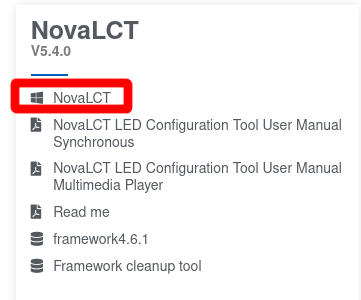
\includegraphics[scale=.9]{NOVALCT_INSTALL.png}
			\caption{\label{fig:NOVALCT_INSTALL}Baixando o executável do NovaLCT}
		\end{figure}
	\item Clique no Executável instalado,
	\item Clique em ``OK'' para conceder permissões ao programa,
	\item Escolha a linguagem,
		\begin{figure}[!htb]
			\centering
			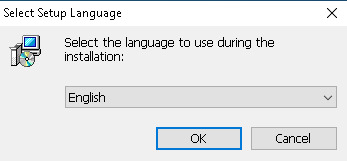
\includegraphics[width=\textwidth]{D1.jpeg}
			\caption{\label{fig:D1.jpeg}Primeira tela do processo de instalação}
		\end{figure}
		\newpage
	\item Aceitar termos de uso,
		\begin{figure}[!htb]
			\centering
			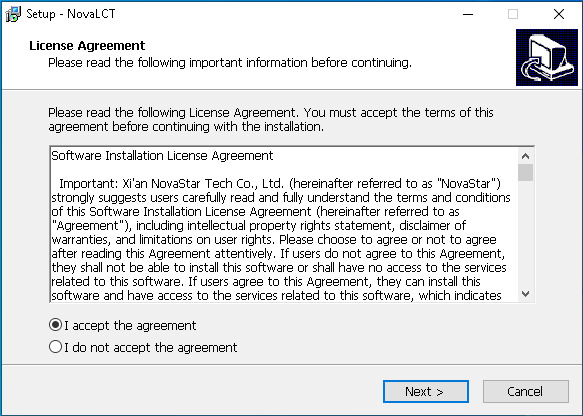
\includegraphics[width=.8\textwidth]{D2.jpeg}
			\caption{\label{fig:D2.jpeg}Segunda tela do processo de instalação}
		\end{figure}
	\item Escolher caminho da instalação,
		\begin{figure}[!htb]
			\centering
			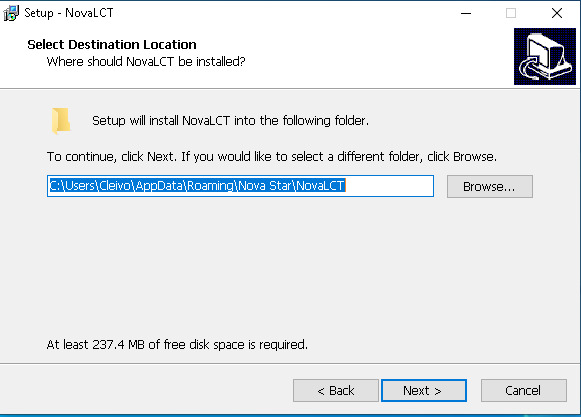
\includegraphics[width=.8\textwidth]{D3.jpeg}
			\caption{Terceira tela do processo de instalação}
		\end{figure}
		\newpage
	\item Escolher caminho do Menu,
		\begin{figure}[!htb]
			\centering
			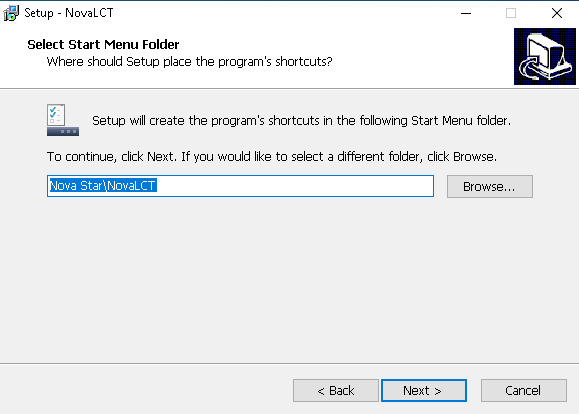
\includegraphics[width=.8\textwidth]{D4.jpeg}
			\caption{Quarta tela do processo de instalação}
		\end{figure}
	\item Escolher criar um ícone na Área de Trabalho,
		\begin{figure}[!htb]
			\centering
			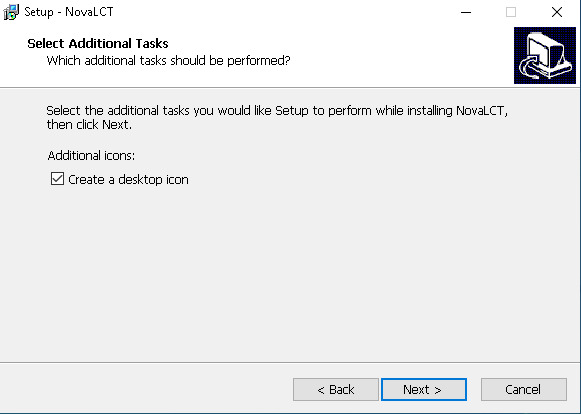
\includegraphics[width=.8\textwidth]{D5.jpeg}
			\caption{Quinta tela do processo de instalação}
		\end{figure}
		\newpage
	\item Clique em ``instalar'',
		\begin{figure}[!htb]
			\centering
			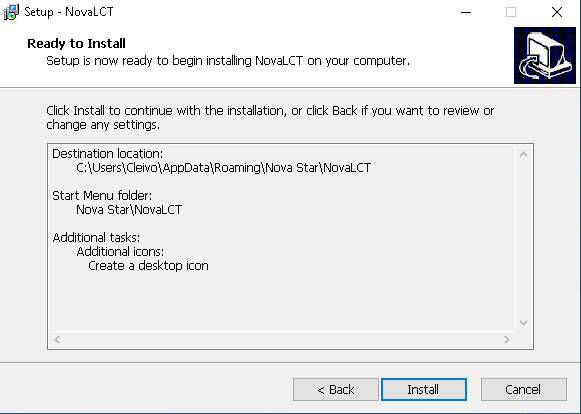
\includegraphics[width=.8\textwidth]{D6.jpeg}
			\caption{Sexta tela do processo de instalação}
		\end{figure}
		\begin{figure}[!htb]
			\centering
			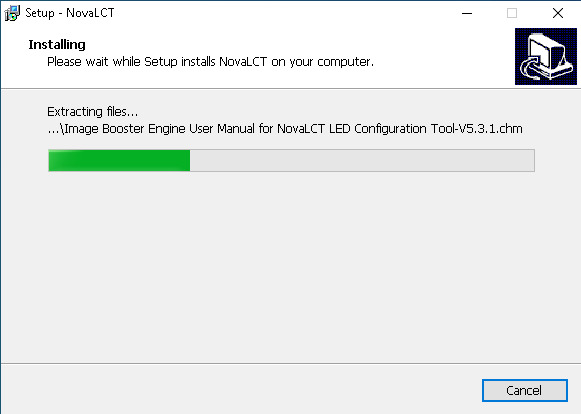
\includegraphics[width=.8\textwidth]{D7.jpeg}
			\caption{Instalação em andamento}
		\end{figure}
		\newpage
	\item Instalando drivers,
		\begin{figure}[!htb]
			\centering
			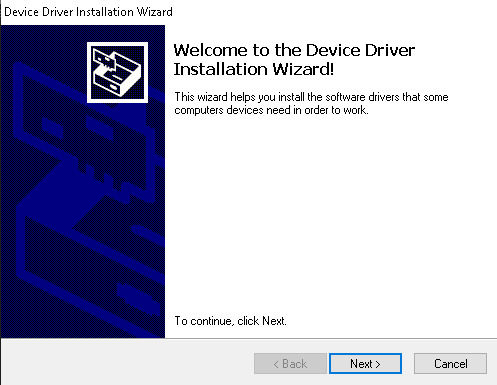
\includegraphics[width=.75\textwidth]{D8.jpeg}
			\caption{Tela inicial do processo de instalação dos drivers}
		\end{figure}
	\item Clique em ``Finish'',
		\begin{figure}[!htb]
			\centering
			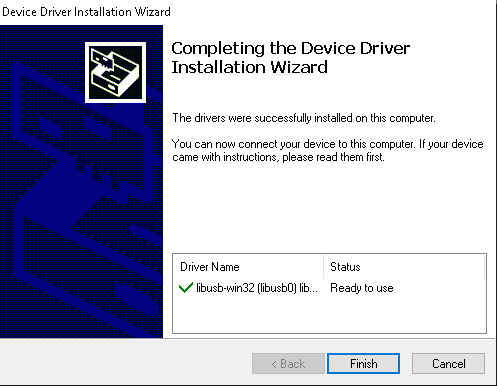
\includegraphics[width=.75\textwidth]{D9.jpeg}
			\caption{Instalando os drivers}
		\end{figure}
		\newpage
	\item Finalize o processo de instalação.
		\begin{figure}[!htb]
			\centering
			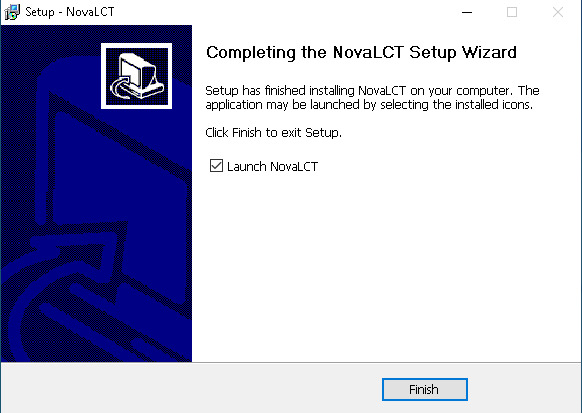
\includegraphics[width=.8\textwidth]{DEnd.jpeg}
			\caption{Última tela do processo de instalação}
		\end{figure}
\end{enumerate}

\newpage
\section{Configurando o software}\label{Configurando o software}
Tendo o software sido instalado com sucesso, ao abri-lo deve-se obter uma tela como a Figura~\ref{fig:CS1.jpeg} abaixo:
\begin{figure}[!htb]
	\centering
	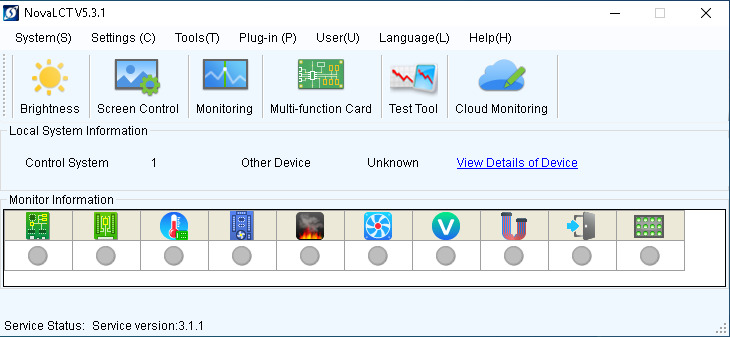
\includegraphics[width=\textwidth]{CS1.jpeg}
	\caption{\label{fig:CS1.jpeg}Tela inicial do software}
\end{figure}

\subsection{Acessando como administrador}\label{Acessando como administrador}
Agora logue como admin, entrando na aba ``User (U)'' e clicando na opção ``Advanced Synchrounus System User Login''.
\begin{figure}[!htb]
	\centering
	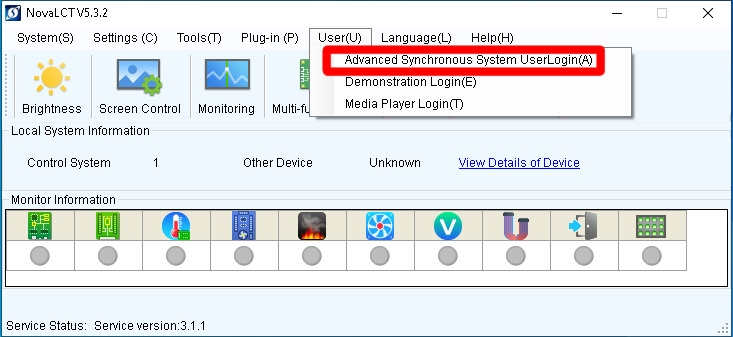
\includegraphics[width=\textwidth]{CS2.jpeg}
	\caption{\label{fig:CS2.jpeg}Aba para efetuar login}
\end{figure}

\newpage
Entre com a senha que por padrão é ``admin''.
\begin{figure}[!htb]
	\centering
	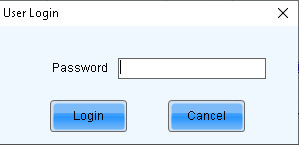
\includegraphics[width=.6\textwidth]{CS3.jpeg}
	\caption{\label{fig:CS3.jpeg}Menu de login}
\end{figure}

\section{Configurando a rede}\label{Configurando a rede}

Quando o software é instalado com sucesso, por dependência instala-se também um gerenciador de rede, o qual é executado junto com o NovaLCT, gerando o seguinte item na barra de tarefas, como vemos na Figura~\ref{fig:barra_de_tarefas.jpeg}:
\begin{figure}[!htb]
	\centering
	
\includegraphics{barra_de_tarefas.jpeg}
	\caption{\label{fig:barra_de_tarefas.jpeg}Ícone do Gerenciador de rede}
\end{figure}

\section{Conexão dos painéis}\label{Conexão dos painéis}
\begin{enumerate}
	\item 
\end{enumerate}

% ----------------------------------------------------------
% Referências bibliográficas
% ----------------------------------------------------------
\cleardoublepage
\bibliography{ref}

\end{document}
